\subsection{Custom Chips}

%Coupling structural with learnt features
\begin{figure*}[!htb]
\centering
\begin{tabular}{@{}c@{} @{}c@{} @{}c@{} @{}c@{}}
\vspace{-5pt}

\includegraphics[width=0.25\linewidth,trim={0 0 0 0},clip]{MissingFigure.pdf} & 
\includegraphics[width=0.25\linewidth,trim={0 0 0 0},clip]{MissingFigure.pdf} & 
\includegraphics[width=0.25\linewidth,trim={0 0 0 0},clip]{MissingFigure.pdf} & 
\includegraphics[width=0.25\linewidth,trim={0 0 0 0},clip]{MissingFigure.pdf}\\[\abovecaptionskip]
\small(a) Original image & \small (b) HOG output & \small (c) Reduced threshold HOG output & \small (d) HOG-CNN output \\
\end{tabular}
\caption{Coupling structured features with learnt features}
\label{tab:tn}
\end{figure*}

\subsection{Brain-like Architectures}
As machine learning workloads become more and more involved, modern architectures beyond von-Neumann are being explored.
IBM's TrueNorth chip consists of 4096 neurosynaptic cores arranged in a 2-D
array occupying 4.3 ${cm^2}$ of area in a 28 nm lowpower CMOS process. This brain-like chip consumes merely 65 mW of 
power while running a typical computer vision application~\cite{truenorth}. Having accelerated some of the key computer vision models using custom fabrics 
like FPGAs and GPUs, we are now looking to map them onto TrueNorth. Figure~\ref{tab:tn} shows the output of the HOG-based person detection when modeled for TrueNorth. 

%TN
\begin{figure*}[!htb]
\centering
%\def\arraystretch{1.5} %
\begin{tabular}{@{}c@{} @{\hspace{2em}}c@{} @{\hspace{2em}}c@{}}
\vspace{-5pt}
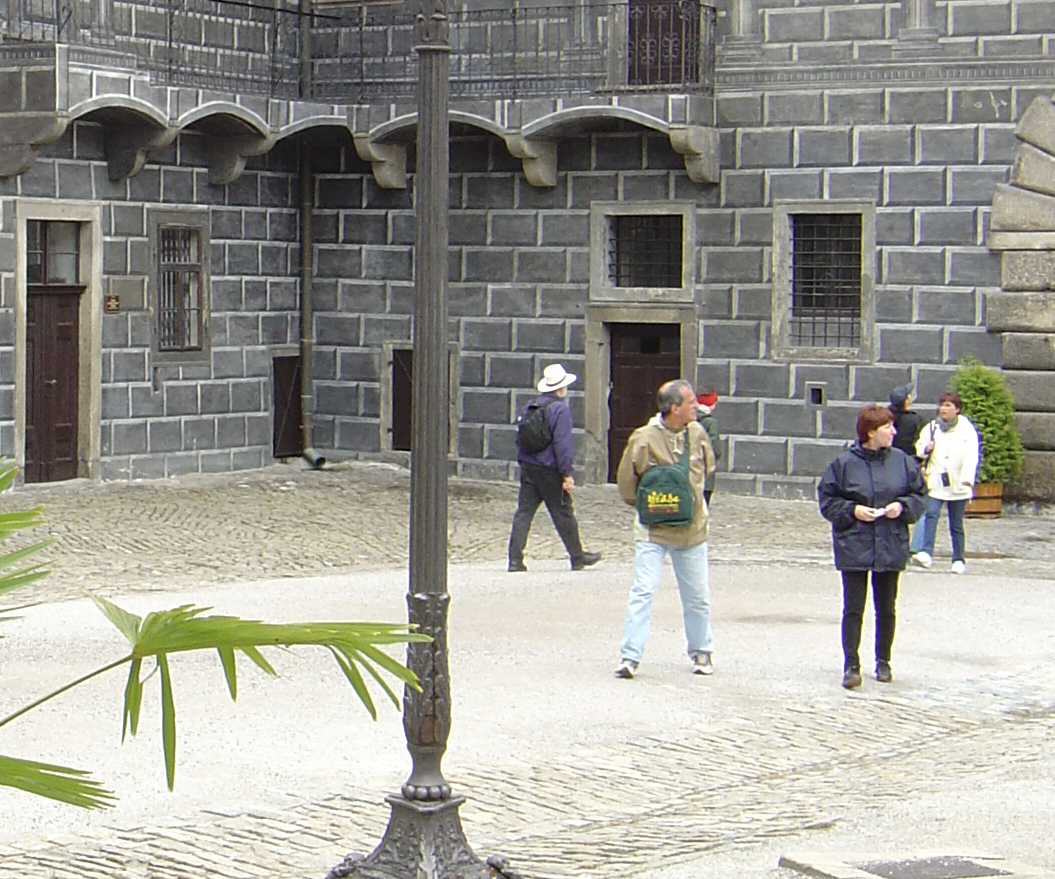
\includegraphics[width=0.29\linewidth,trim={0 0 0 0},clip]{tn_input_46.png} & 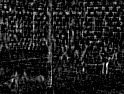
\includegraphics[width=0.32\linewidth,trim={0 0 0 0},clip]{tn_dotp_46.jpg} & 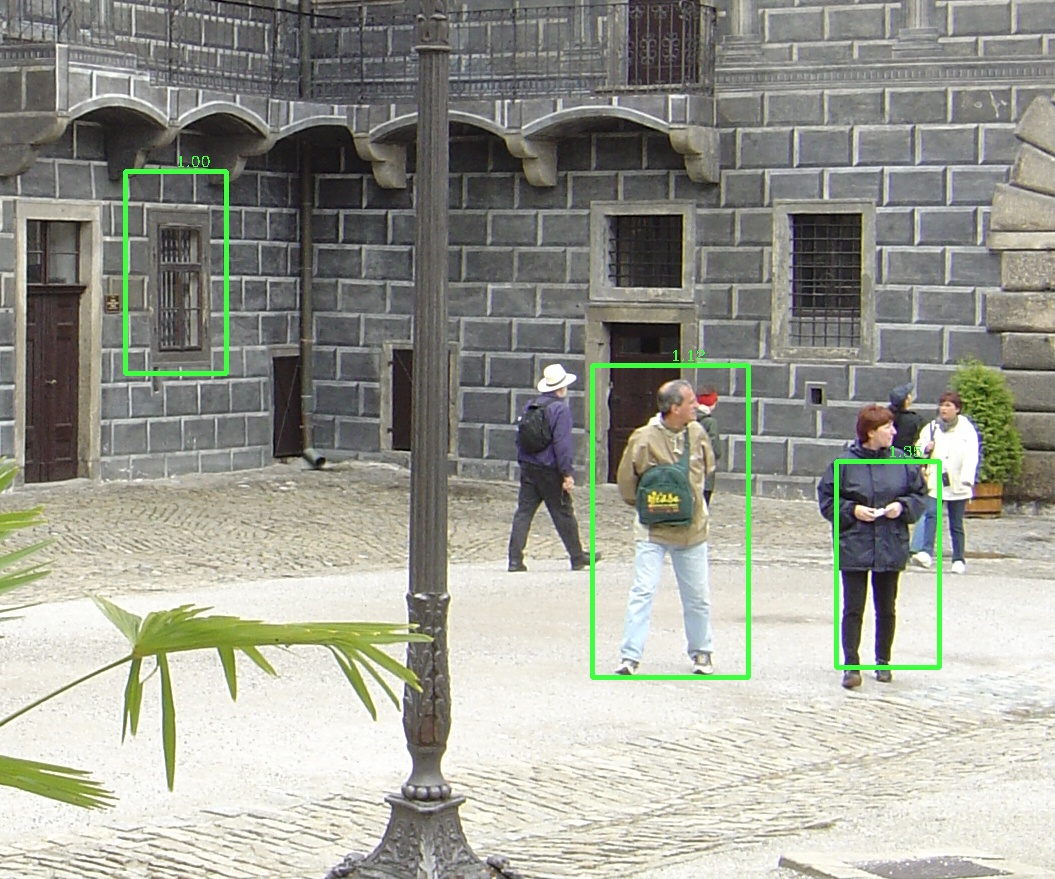
\includegraphics[width=0.29\linewidth,trim={0 0 0 0},clip]{tn_detection_46.jpg}\\[\abovecaptionskip]
\small(a) Original image & \small (b) Dot Product & \small (c) Detections \\
\end{tabular}
\caption{Mapping HOG to True North}
\label{tab:tn}
\end{figure*}

\subsection{Emerging Devices}

